\section{Experiments}
\label{sec:experiments}

\subsection{Experimental Setup}

% Harness-only evolution, with the frozen model never updated. The seven-domain main results
% use \textbf{Qwen3.6-27B}; the cross-model study (Table~\ref{tab:crossmodel}) additionally
% evolves two further frozen models on AppWorld, \textbf{Qwen3.5-397B-A17B-GPTQ-Int4} and
% \textbf{Gemini~3 Flash} (a non-Qwen API model). The evolver's diagnoser $D$ (a separate, stronger model, $D\neq M$) is Claude Opus~4.8,
% driven through Claude Code to run the loop end-to-end (\S\ref{sec:labor});
% $D$ is reported for reproducibility, not required.
% \textbf{Seven domains}: terminal-bench-2~\citep{merrill2026terminalbench} (TB2), the
% EvoAgentBench suite~\citep{gao2026evoagentbench} (LiveCode, Omni-MATH, BrowseComp+, GDPval,
% SWE-bench), and AppWorld~\citep{trivedi2024appworld}. Six are
% credited on disjoint training/test splits (Table~\ref{tab:main}, top six); the
% seventh (SWE-bench) is preliminary (bottom row) and analyzed at the end of this section. $K{=}3$ attempts per task;
% per-task success (Pass@1) with denominator $=$ total tasks (\S\ref{sec:gates}). The
% train-selected harness is scored \emph{once} on the test, never consulted during
% evolution (\S\ref{sec:protocol}). Verifiers are of two kinds: \emph{deterministic} task-success checks (TB2 harbor with a
% timeout-fair overlay; LiveCode lcb\_runner; AppWorld task-success) and
% \emph{model-based} scorers (Omni-MATH and BrowseComp+ by LLM judge, pass $=$ reward $1.0$;
% GDPval by a gpt-4o rubric proxy, pass $=$ reward $\ge 0.6$).
We evaluate HarnessBank on seven domains with disjoint train/test splits: Terminal-Bench-2
(TB2)~\citep{merrill2026terminalbench}, five from EvoAgentBench (LiveCode, Omni-MATH,
BrowseComp+, GDPval, SWE-bench)~\citep{gao2026evoagentbench}, and
AppWorld~\citep{trivedi2024appworld}. All experiments evolve the harness only, with the
backbone frozen; by default \textbf{Qwen3.6-27B}. Claude Opus~4.8 serves as the evolver
agent. The primary metric is per-task success (Pass@1) averaged over $K{=}3$ attempts per
task. We compare against two state-of-the-art harness self-evolution methods,
GEPA~\citep{agrawal2026gepa} and DGM~\citep{zhang2026dgm}.
%Candidate and vanilla harnesses are compared using task-level paired differences, and a held-out gain is credited only when it is positive and clears the paired-$2\sigma$ threshold ($z\geq1.96$).
%
%We additionally report the absolute percentage-point improvement and the retention ratio, defined as the held-out improvement divided by the corresponding training improvement.



\begin{figure*}[t]
  \centering
  \IfFileExists{figures/fig-baselines.pdf}{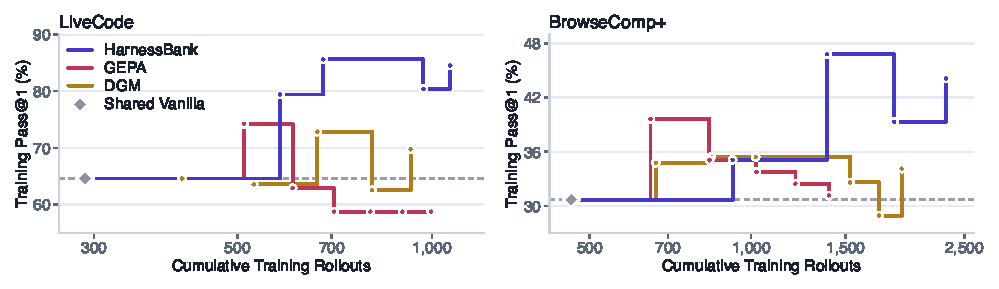
\includegraphics[width=0.9\textwidth]{figures/fig-baselines.pdf}}{\figplaceholder{Fig.~\ref{fig:baselines}: export figures/fig-baselines.pdf}}
  \caption{Evolution trajectories (frozen Qwen3.6-27B): every harness produced, in order,
against cumulative rollouts (log scale), from a shared vanilla (diamond). No method climbs
monotonically --- GEPA's first candidate is its best on both domains. Training scores do
\emph{not} rank methods; ranking is decided once on the sealed test
(Figure~\ref{fig:testbars}).}
  \label{fig:baselines}
\end{figure*}

\subsection{Main results}

The train-selected harness improves over vanilla on \emph{every} test set, and every gain
clears the paired-$2\sigma$ bar (Table~\ref{tab:main}), from $+9$ to $+15.4$\%. The
recurring win is harness-level recovery of the frozen model's dominant failure mode (empty
``thinking-runaway'' turns), on several domains stacked with a verify-finalize self-check
(VF); our running example BrowseComp+ is one such recombination, credited at $+13.9$\%.

The seventh domain, SWE-bench, runs the same loop on a $101/26$ split: its harness is
strongly credited on training ($+13.9$\%, $n{=}101$) and lifts the test ($+5.1$\%), but
at $n{=}26$ even a real $+5$\% effect sits below the bar ($z{=}0.78$), so we report it as
\emph{preliminary} --- small-$n$ noise, not overfitting.

\begin{table*}[t]
\centering
\footnotesize
\setlength{\tabcolsep}{3pt}
\caption{Main results of HarnessBank on seven benchmarks. \emph{Vanilla} denotes the harness at initialization and \emph{Evolved} denotes the self-evolved harness by HarnessBank. Parentheses $=$ gain over vanilla (\%). Ret. $=$
test$\div$training gain. }
\label{tab:main}
\begin{tabular}{llccccccc}
\toprule
 & & \multicolumn{2}{c}{Training Pass@1} & \multicolumn{2}{c}{Test Pass@1} & & \multicolumn{2}{c}{Test Pass@3} \\
\cmidrule(lr){3-4}\cmidrule(lr){5-6}\cmidrule(lr){8-9}
Benchmark & Domain & Vanilla & Evolved & Vanilla & Evolved & Ret. & Vanilla & Evolved \\
\midrule
TB2               & Terminal Operation  & $37.7$ & $44.0$ ($+\phantom{0}6.3$) & $36.1$ & $\mathbf{45.4}$ ($+\phantom{0}9.3$) & $148\%$ & $52.8$ & $58.3$ ($+\phantom{0}5.5$) \\
LiveCode          & Code Generation     & $64.6$ & $85.6$ ($+21.0$) & $58.1$ & $\mathbf{71.8}$ ($+13.7$) & $65\%$ & $66.7$ & $79.5$ ($+12.8$) \\
Omni-MATH         & Math Reasoning      & $78.4$ & $91.1$ ($+12.7$) & $54.3$ & $\mathbf{66.0}$ ($+11.7$) & $92\%$ & $65.0$ & $75.0$ ($+10.0$) \\
BrowseComp+       & Web Research        & $30.7$ & $46.8$ ($+16.1$) & $16.9$ & $\mathbf{30.8}$ ($+13.9$) & $86\%$ & $33.8$ & $49.2$ ($+15.4$) \\
GDPval            & Knowledge Work      & $73.6$ & $82.0$ ($+\phantom{0}8.4$) & $43.7$ & $\mathbf{52.9}$ ($+\phantom{0}9.2$) & $110\%$ & $58.6$ & $67.2$ ($+\phantom{0}8.6$) \\
AppWorld          & App \& API Control  & $51.9$ & $69.7$ ($+17.8$) & $41.3$ & $\mathbf{56.7}$ ($+15.4$) & $86\%$ & $67.3$ & $75.6$ ($+\phantom{0}8.3$) \\
SWE-bench         & Repo-Level Bug Fix  & $55.4$ & $69.3$ ($+13.9$) & $47.4$ & $\mathbf{52.6}$ ($+\phantom{0}5.1$)          & $37\%$ & $61.5$ & $69.2$ ($+\phantom{0}7.7$) \\
\bottomrule
\end{tabular}
\end{table*}



\subsection{Comparison with Existing Methods}
\label{sec:baselines}

We compare HarnessBank against two state-of-the-art methods: GEPA~\citep{agrawal2026gepa}, which is
\emph{prompt-only}, and the Darwin G\"odel Machine (DGM)~\citep{zhang2026dgm}, which self-modifies
openly but \emph{ungated}. Both run under HarnessBank's protocol --- same frozen Qwen3.6-27B
as task agent \emph{and} proposer, same splits, same paired-$2\sigma$ ruler --- on comparable
budgets ($780$--$2{,}310$ rollouts each, within $2.1\times$ on any domain), with GEPA outspending
us on two domains and DGM on one (Figure~\ref{fig:baselines}).

\begin{figure}[t]
  \centering
  \IfFileExists{figures/fig-testbars.pdf}{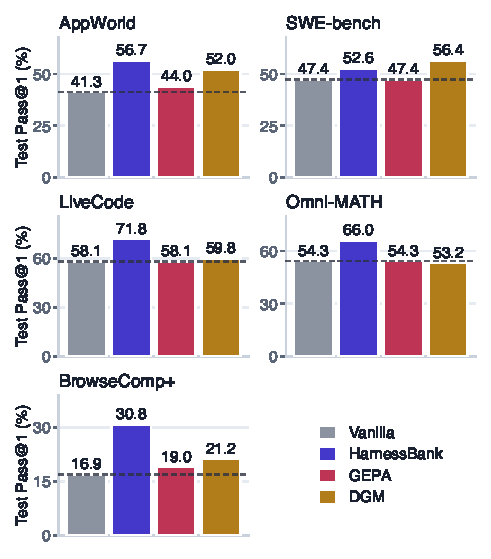
\includegraphics[width=\columnwidth]{figures/fig-testbars.pdf}}{\figplaceholder{Fig.~\ref{fig:testbars}: export figures/fig-testbars.pdf}}
  \caption{Test Pass@1 ($K{=}3$) of different methods. Dashed lines denote the performance of the vanilla harness. }
  \label{fig:testbars}
\end{figure}

Across the five sealed tests of Figure~\ref{fig:testbars}, HarnessBank is credited on
\emph{four} (SWE-bench falls short only at $n{=}26$), DGM on \emph{one}, and GEPA on
\emph{none}.

GEPA finds \emph{no} variant beating its seed on LiveCode in $47$ iterations:
thinking-runaway is not prompt-addressable. Where its search returns no train-improving
candidate it ships vanilla, so three of its five cells sit at the baseline. On AppWorld,
whose win surface \emph{is} partly prompt-expressible, its training gain washes out on the
sealed test ($+2.8$, $z{=}0.97$).

DGM clears the bar once: AppWorld, $+10.7$\% ($z{=}3.00$). Its other cells show the cost
of selecting without a significance gate. On LiveCode it picks its best of $15$ generations
on a $15$-task $K{=}1$ spike ($0.733$, regressing to $0.533$ on re-evaluation) and lands
uncredited ($z{=}0.66$); on Omni-MATH the harness it ships is \emph{worse} than vanilla
($-1.1$\%) --- an ungated loop can deploy a regression.

The contrast is thus not search effort but what the edits can reach and what survives the
gates. On SWE-bench, the one domain where a baseline scores highest, neither is credited and
$n{=}26$ cannot separate them.


\subsection{Significance and Generalization}
\label{sec:sig}

All six test gains are \emph{credited}: each per-task paired difference clears
$z\!\ge\!1.96$ on tasks the evolving agent never saw ($p$ from $<10^{-4}$ to $0.033$;
AppWorld strongest at $z{=}6.44$, $n{=}168$). Each is a \emph{single} comparison (the
train-selected winner scored once on held-out tasks), so the many candidate comparisons
during evolution cannot inflate it. The gate is two-sided: on TB2 it culled a significantly
\textbf{negative} candidate ($-6.4$\%).

Test lift retains $65$--$148\%$ of train lift; none collapses. Two benchmarks exceed their
training gain and three retain $86$--$92\%$; LiveCode, whose training gain is the largest in
the suite, retains $65\%$. Retention is a ratio of two
noisy estimates that a small denominator inflates (GDPval's $110\%$ divides by $+8.4$\%,
LiveCode's $65\%$ by $+21.0$\%), so we do not treat it as a test: the load-bearing claim is
the credited held-out gain.

pass@3 also rises on \emph{every} credited domain ($+5.5$ to $+15.4$\%), so the harness
\emph{expands the set of solvable tasks}, not just the per-attempt hit rate; pass@1 remains
our primary metric.

\subsection{Diagnosis and Cost}

Two pathologies recur, each fixed by a distinct \textsc{runtime} mechanism:
\emph{thinking-runaway empty} turns, fixed by selective recovery, and
\emph{premature/unverified finalization}, fixed by a verify-finalize self-check. On five
domains a single pathology dominates $49$--$88\%$ of vanilla failures and the matched
mechanism is credited on the test, under both deterministic and judge-based verifiers ---
evidence of a \emph{true} failure mode of the frozen model rather than a scoring artifact.
The two domains with heterogeneous failure maps still yield credited and preliminary
patches.



\why{} is an LLM-assigned \emph{hypothesis}, not ground truth: on AppWorld the loop
misdiagnosed a capability limit as a knowledge gap, and the gate rejected the proposed patch
(its own target task $0/24 \to 0/24$, $p{=}1.0$). Because \why{} only steers which candidates
to try while credit comes solely from the gate, a wrong label costs at most a rejected
candidate, never a bad harness.

\subsection{Cross-Model Dissociation}

Thinking-runaway dominates four of six domains, but the loop is not re-fixing one
qwen3.6-27B quirk. The recurring win is a \emph{model} property (reasoning-budget overrun):
the credited mechanism disables thinking only \emph{after} a runaway, and on LiveCode neither
a $16\times$ token budget nor a blanket thinking-off toggle reproduces its gain. Cold-started
on other models the loop evolves \emph{their own} credited harnesses, each targeting that
model's distinct pathology (Table~\ref{tab:crossmodel}).

The patches follow a \emph{pathology$\to$patch matching law}: each model's dominant pathology
draws a patch that helps it and not models with a different one. On AppWorld the 27B fails by
empty ``engagement'' turns, fixed by verify-finalize, whereas the 397B and
\textbf{Gemini~3~Flash} make careless errors, fixed by a submit-verify checklist; Gemini
reproduces the careless$\to$checklist match ($+13.5$\%, $z{=}4.15$), extending the law
across \emph{families}. Off the diagonal the mismatched patch is near-zero on the Qwen pair
($+0.2$, $+1.2$); on Gemini verify-finalize still gains $+5.8$, a gradient rather than a
switch because it shares a verify step with the checklist.

Omni-MATH supplies the converse. The two Qwen generations \emph{share} the pathology
(thinking-runaway on long competition math) and the 27B-evolved stack transfers nearly
loss-free ($+11.7$ native, $+11.0$ transferred, both credited). Gemini reasons too
\emph{little} instead, so the transplanted recovery never fires ($-1.5$) while its matched
patch turns the \emph{same} lever the other way, to saturation ($+15.3$, credited). Turning
it the wrong way is not merely neutral but harmful: $-15.7$ when stacked on the evolved 397B
harness. The two families need one lever turned in opposite directions: a credited harness is
a correction fitted to the model, not a universally good setting.

\begin{table}[t]
\centering
\footnotesize
\setlength{\tabcolsep}{3.5pt}
\caption{Cross-model matching law: Test $\Delta$Pass@1 (\%). \textbf{Bold} $=$ matched
patch (paired-$2\sigma$). A/B $=$ VF\,/\,SV on AppWorld, 27B-stack\,/\,raise-reasoning on
Omni-MATH.}
\label{tab:crossmodel}
\begin{tabular}{lllcc}
\toprule
Domain & Model & Dominant Failure & A & B \\
\midrule
AppWorld  & 27B    & Empty Engagement  & $\mathbf{+15.4}$ & $+1.2$ \\
          & 397B   & Careless          & $+0.2$           & $\mathbf{+13.6}$ \\
          & Gemini & Careless          & $+5.8$           & $\mathbf{+13.5}$ \\
\midrule
Omni-MATH & 27B    & Thinks Too Much   & $\mathbf{+11.7}$ & $+1.7$ \\
          & 397B   & Runaway (Shared)  & $\mathbf{+11.0}$ & $+0.7$ \\
          & Gemini & Thinks Too Little & $-1.5$           & $\mathbf{+15.3}$ \\
\bottomrule
\end{tabular}

\end{table}


\subsection{Ablation Study}

Train selection is a \emph{lower bound} on what generalizes: on GDPval a variant ranked
below the winner on train scored \emph{highest} on test ($+11.5\%$ vs.\ $+9.2$\%) --- hence
crediting on held-out data.

Does the paired-$2\sigma$ gate matter, or would prior work's ``mean improves'' rules suffice?
Table~\ref{tab:gates} ablates it on TB2 along what gets deployed, what enters the archive,
and whether the loop can stop. Deployment is unchanged (train-argmax already picks VF), but
two noise mechanisms enter as elites --- one inert, its activation beacon never firing ---
and false elites then seed parents, spending future budget on noise. Termination is decisive:
on post-convergence rounds with neutral candidates, phantom progress appears in
$62$--$76\%$ of rounds under single-run or $K{=}3$-mean crediting, so the loop stops only at
the cap, whereas paired-$2\sigma$ stops at the $10$-round floor.



\begin{table}[t]
\centering
\footnotesize
\setlength{\tabcolsep}{3pt}
\caption{Ablation results on TB2. Rows below HarnessBank denote modified variants.
\emph{False elites} $=$ evolved harnesses whose gains in the test cannot be distinguished from
noise; $>20$ (cap) $=$ the stop rule is never met.}
\label{tab:gates}
\begin{tabular}{lccc}
\toprule
TB2 Configuration & Test Pass@1 & False Elites & Rounds \\
\midrule
\textbf{HarnessBank} ($K{=}3$, $2\sigma$) & $\mathbf{45.4}$ & $\mathbf{0}$ & $\mathbf{10.0}$ \\
w/o $2\sigma$                       & $\pm 0.0$ & $+2$ & $>20$ (cap) \\
w/o confirm $+$ $2\sigma$           & $-1.6$ & $+3$ & $>20$ (cap) \\
Vanilla                             & $-9.3$ & --- & --- \\
\bottomrule
\end{tabular}
\end{table}

Two signs the archive earns its keep. First, on most domains the credited harness
stacks mechanisms drawn from more than one cell, and it is the per-cell elite that
keeps the second mechanism alive long enough to be recombined at all. Second, accepted edits
span all four levers rather than prompts alone. The diversity axis is \emph{semantic} rather than
per-task by design: an archive keyed on tasks would preserve harnesses indexed by the very
tasks used to select them, which overfits by construction.

